\section{\mbox{Deathtime-Based Garbage Collection}}\label{sec:GDT}
Out‑of‑place systems require garbage collection (GC).
When a new version of a page is written, the previous version becomes invalid; 
stale data accumulates until capacity is exhausted.
We first explain how GC affects DB WAF, then introduce \emph{Grouping by Death Time} (GDT), 
which reduces WA for skewed workloads.

\subsection{Database-Level Write Amplification and GC}\label{sec:gc}

\module{GC overview.}
GC reclaims space occupied by stale pages, as illustrated in \cref{fig:gc}.  
Storage is divided into {\tt zones}, each containing multiple pages (eight in the figure), defining the GC granularity.  
When a new page is written, it is appended to a selected zone with available space, and the mapping table is updated while the old version is marked invalid.  
Over time, zones accumulate a mix of valid and invalid pages.
During GC, the garbage collector selects a \emph{victim zone} containing both valid and invalid pages (\ding{182}).  
In \cref{fig:gc}, 6 of 8 pages are valid, giving a 75\% valid ratio.
To reclaim space, valid pages not in memory are loaded (\ding{183}), compacted (\ding{184}), and rewritten (\ding{185}).
This copyback process reclaims space for two new writes (\ding{186}) but incurs WA, as six pages must be rewritten.
Garbage-collecting zones with more valid data therefore naturally yields higher WA.

\module{GC valid ratio drives DB WAF.}
The GC copyback drives DB WAF, as more pages are rewritten than originally requested.
WAF depends on the valid ratio of the victim zone in each GC cycle.
In \cref{fig:gc}, 75\% of the pages are valid, yielding a WAF of $1/(1-0.75)=4$, since 75\% of the data must be copied to free 25\% of the space.

\module{Skewed workloads require better GC.}
A common victim selection strategy for GC (\ding{182} in \cref{fig:gc}) is greedy; choosing the zone with the fewest valid pages.
This is optimal under uniform random workloads~\cite{DBLP:journals/cacm/LangeNY23, ssdiq}.
However, real-world workloads are typically skewed~\cite{DBLP:journals/tos/YadgarGJS21}, 
making greedy GC suboptimal~\cite{DBLP:journals/pvldb/KangCOL20, ssdiq}, as skew colocates hot and cold pages within zones, raising valid-page ratios and thus WA.

\module{DBMSs know better.}
To improve GC under skew, prior work proposes advanced GC and placement schemes---classifying data by hotness~\cite{DBLP:journals/pvldb/KangCOL20}, expected lifetime~\cite{dtp, DBLP:conf/fast/WangLLOSH22}, or based on spatial and temporal locality~\cite{DBLP:journals/pvldb/YuMKLMK22, DBLP:journals/pe/Houdt14, DBLP:conf/hotstorage/ShafaeiDF16}.
By grouping pages along these dimensions, these methods aim to reduce valid ratios in victim zones.
However, these techniques generally target SSD firmware or filesystems, which lack visibility into upper-layer workloads~\cite{Multistream, flashalloc, fdp}, limiting their ability to perform workload-aware GC.
In contrast, database systems possess richer workload and data semantics, making them well positioned to exploit intelligent GC schemes~\cite{DBLP:conf/sigmod/OzmenSSD10}.



\begin{figure}
    \centering
    \begin{subfigure}[t]{0.49\linewidth}
        \centering
        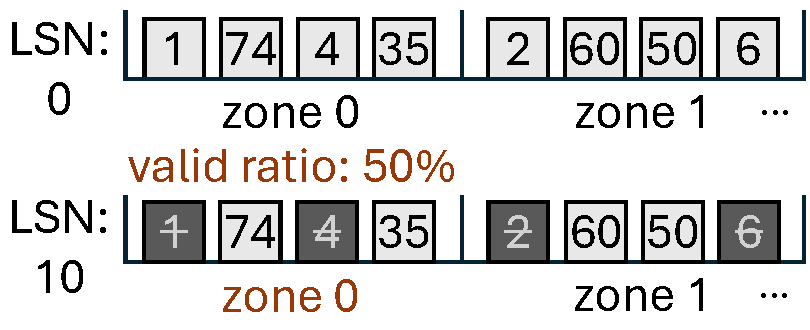
\includegraphics[width=0.95\linewidth]{figures/edtbefore.pdf}
        \caption{Random placement}
        \label{fig:beforegdt}
    \end{subfigure}
    \hfill
    \begin{subfigure}[t]{0.49\linewidth}
        \centering
        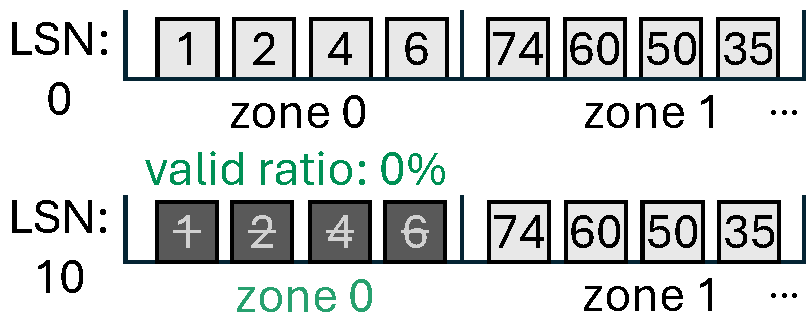
\includegraphics[width=0.95\linewidth]{figures/edtafter.pdf}
        \caption{Placement using GDT}
         \label{fig:aftergdt}
    \end{subfigure}
    \caption{Impact of different placement strategies on WA\\
    ({\setlength{\fboxsep}{1pt}\raisebox{0pt}{\fbox{\tiny 1}}} denotes a page with deathtime 1.)}
    \vspace{-3mm}  % reduces vertical space below the figure
    \label{fig:gdt}
\end{figure} 



%%%%%%%%%%%%%%%%%%%%%%%%%%%%%%%%%%%%%%%%%%%%%%%%%%%%%%%%%%%%%%%%%%%%%%%%%%%%%%%%%%%%%%%%%%%%%%%%%%%%%%%%%%%%%%%%%%%%%%%%%%%%%%%%%%%%%%%%%%%%%%%%%
\subsection{Grouping Pages By Deathtime}
We introduce \emph{Grouping by Death Time} (GDT)~\cite{DBLP:journals/cacm/LangeNY23,DBLP:conf/eurosys/HeKAA17} into DB GC to reduce DB-WAF.
GDT uses database semantics to estimate each page’s \emph{deathtime} (invalidation time).
This classification guides placement and GC, grouping pages that die together into the same zone and thereby reducing WA during reclamation (\ding{184}--\ding{186} in \cref{fig:gc}).

\module{Optimization: placing pages with similar deathtime per zone.}
GDT packs pages with similar deathtimes into the same zone so they are invalidated together. 
In \cref{fig:gdt}, eight pages with deathtimes 1, 2, 4, 6, 35, 50, 60, and 74 are written at LSN~0. 
If placed randomly (\cref{fig:beforegdt}), zones mix short- and long-lived pages, yielding a 50\% valid ratio at LSN~10 when greedy GC triggers. 
With GDT (\cref{fig:aftergdt}), pages are grouped by deathtime, so at LSN~10, victim zone~0 has no valid pages, eliminating WA for that cycle. 
Thus, aligning placement with deathtime substantially reduces GC-induced WA.

\module{Using write timestamps for deathtime estimation.}
To apply GDT, the system must estimate each page’s deathtime before writing it to SSD.
We extend each page header with a write timestamp, updated whenever the page is persisted~\cite{DBLP:journals/pvldb/VohringerL23}, and maintain a write history (WH) of the last $n$ timestamps (e.g., 4). GC writes do not update WH.
We estimate the next write time as: $\textit{EDT} = \textit{current\_lsn} + \frac{\textit{WH}_n - \textit{WH}_1}{n - 1}$,
extrapolating recent write intervals to predict when the page will next be overwritten.
For initial writes, pages are grouped by B-tree index ID to colocate pages with similar access patterns~\cite{DBLP:conf/sigmod/OzmenSSD10}.

\module{GDT-based placement strategy.}
When a batch of pages is written upon eviction, GDT first computes each page’s EDT.
Pages are then grouped and page-packed so that each group contains pages with similar deathtimes.
For each group, the strategy selects the zone whose existing pages have the closest average EDT; if no such zone is active, a new zone is opened.
This concentrates pages with similar deathtimes into the same zone.

\module{GDT-based GC.}
GDT placement is effective only when paired with GDT-aware GC; otherwise, GC writes and normal writes may intermix.
GC greedily selects victim zones until their cumulative invalid pages free the space of one zone.
All valid pages in these victims are loaded, sorted in descending EDT, grouped and packed, and written to an open zone with a matching EDT when possible; otherwise, they remain in their original zone.
Pages that are never rewritten (e.g., read-only pages) are assigned the maximum EDT to be treated as the coldest data.
This replacement during GC also compensates for initial EDT mispredictions.

\module{Reassigning EDT ranges after GC.}
After each GC cycle, zones may be full, partially full, or empty.
Empty and partially full zones are made available for normal writes.
The newly emptied zone is assigned the minimum EDT range, drawing short-lived pages; partially full zones naturally attract warm pages; and full zones retain the coldest pages.
This preserves aligned invalidation times within each zone, even after going through GC cycles.


% \module{Providing locality with GDT-based placement.}
% In addition to grouping PIDs with similar EDTs within a write batch, EDT is also used when selecting a {\tt zone} to place the write request.
% When deciding which zone to write to, we check the average EDT of the zone and place the page-packed PIDs in the zone whose average EDT is closest to the group's EDT.
% This reduces the valid ratio during GC by grouping PIDs with similar EDTs both within the buffer pool and at the storage layer.

% Besides reducing WA during GC, placing PIDs with similar EDTs in the same zone is beneficial because they are likely to be accessed during similar periods.
% PIDs in the same zone naturally exhibit temporal locality.
% Adopting this strategy improves spatial locality for PIDs with temporal locality, even with out-of-place writes.
% This is beneficial because the database buffer cache can take advantage of this spatial locality.
% When GC occurs, valid PIDs in the victim zone---previously not in the cache---are fetched from the SSD (\ding{184} in \cref{fig:gc}).
% Even if still valid, these PIDs are likely to be accessed soon due to their close EDT, meaning they are expected to be written soon.
%Thus, reading them into memory is not redundant but serves as prefetching for future transactions.

